\scanpage{3}
\mspage{2}
sommets, y compris ceux \deleted{\unsure{des deux}}\inserted{incidents} aux faces supercritiques, sont d'ordre $4$ --- les sommets sur une telle face $F_i$ correspondent aux \inserted{$2n_i$} arêtes \unsure{simplement} incidentes de $D_i$. Pour l'étude des ``bouts libres'' créés, supposant pour fixer les idées $\Sigma$ stable, on trouve suivant la parité de $n$:

a) $n$ pair, alors chaque face sous-stable donne \uline{deux} bouts libres placés aux extrémités de l'arête d'incidence, et chaque face stable qui touche $F_i$ donne de plus un bout libre cela fait donc
\[
2(2(n-1))+2(n-1)=6(n-1)
\]
bouts libres, ça fait un peu beaucoup.

b) $n$ impair, alors on trouve que chaque face sous-stable adjacente $1$ bout libre (au milieu de l'arête incidente commune), et $0$ sur les faces stables \unsure{juxtaincidentes}, en tout donc $2(n-1)$ bouts libres --- c'est juste ce qu'il faut pour espérer les raccorder, de façon à avoir \inserted{exactement} une des cartes de $(X,\Sigma)$ ``Affinisé'' par $D_i$.

\margin{\uline{NB} Pour le raccord de la face supercritique avec les faces sous-stables adjacentes, on doit encore définir sur $\widetilde D_i$ \deleted{des} (image inverse de $D_i$ dans $\widetilde X$) des \uline{arcs de générisation} \deleted{canoniques}\inserted{autour des} \deleted{les deux} sommets \deleted{\unsure{de}} $\widetilde D_i$, qu'on choisit de longueur combinatoire $1$ --- ce sont donc les arêtes de la subdivision cellulaire de $\widetilde D_i$ dont \unsure{ces celles données} par les les sommets. Non c'est mal dit, il vaut mieux prendre $\widetilde D_i$ \unsure{rev.} des vis de $D_i$, et définir l'arc de générisation rel\unsure{f} à une position relative sous-stable voisine de $D_i$, comme sur la figure ci-contre avec un arc de long $1$ équidistant des deux sommets sur $\widetilde D_i$ correspondant à $s$, et du côté où se trouve la p.r. $D$}
\figure{%
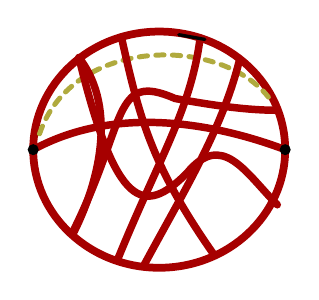
\begin{tikzpicture}[x=1cm,y=1cm,line cap=round]
\draw[red!65!black,line width=2.8pt] (0,0) ellipse(1.6 and 1.5);
\draw[yellow!65!black,dashed,line width=1.8pt] (-1.52,.2)..controls(-1.1,1.45)and(.8,1.45)..(1.4,.65);
\draw[red!65!black,line width=2.7pt] (-1.6,0)..controls(-.5,.6)and(.8,.3)..(1.6,0);
\draw[red!65!black,line width=2.7pt] (-1.02,1.17)..controls(-.5,.5)and(-.8,-.5)..(-1.1,-1.08) (-.48,1.43)..controls(-.25,.4)and(-.1,-.2)..(.7,-1.34) (.52,1.42)..controls(.4,.5)and(.0,-.1)..(-.53,-1.4) (1.02,1.14)..controls(.8,.25)and(.3,-.55)..(-.2,-1.48);
\draw[red!65!black,line width=2.7pt] (-1.1,-1.05)..controls(-.4,.35)and(-.6,1)..(.2,.65)..controls(.75,.55)and(1.15,.5)..(1.5,.5);
\draw[red!65!black,line width=2.7pt] (-1.02,1.17)..controls(-.55,-.75)and(-.2,-.85)..(.35,-.3)..controls(.8,.25)and(1.1,-.3)..(1.5,-.7);
\fill(-1.6,0)circle(2pt);\fill(1.6,0)circle(2pt);\draw[very thick](.25,1.46)--(.58,1.4);
\end{tikzpicture}%
}

Le cas $n$ impair est satisfaisant, mais pas le cas pair tel quel, car il y a alors redondance des bouts libres. Une façon de s'en tirer dans tous les cas, c'est de \deleted{\unsure{partir}}\inserted{partir de} la carte $\mathcal X_0$, et de la modifier en remplaçant chaque sommet supercritique $s$ par un petit disque supercritique.
\deleted{Le nb} Dans le cas $n$ \unsure{pair} chaque face sous-stable incidente à $s$ contribue $\unsure{1|0}$ bout libre, et chaque face stable incidente $1$ bout, et c'est l'inverse si $n$ est impair, donc en tout il y aura $2(n-1)$ bouts libres \deleted{\unsure{et}} qui aboutissent en $F_s$, et \deleted{\unsure{si je raccorde les bouts}}\inserted{le polygone combinatoire qu'ils forment est} can. hom. à celui obtenu sur $\widetilde D_i$ --- d'où une
\margin{2}
